\documentclass{article}

% Math packages
\usepackage{amsthm, amssymb, enumitem}

% Margins settings
\usepackage[margin=1.2in]{geometry}

% Bracket notation (quantum computing/information)
\usepackage{tikz}
\usetikzlibrary{quantikz}
\usepackage{braket}

% Spacing
\usepackage{parskip}
\usepackage{centernot}

% Required for inserting images
\usepackage{graphicx}
\graphicspath{{./Figures/}}

% Hyperlinks
\usepackage[colorlinks=true, allcolors=blue]{hyperref}

% Header
\usepackage{fancyhdr}
\pagestyle{fancy}
\lhead{October 30th, 2024}
\chead{Optimization for Data Science}
\rhead{University of Waterloo}

% Custom commands
\newcommand{\R}{\mathbb{R}}
\newcommand{\E}{\text{E}}
\newcommand{\dom}{\text{dom}}
\newcommand{\ds}{\displaystyle}
\newcommand{\indep}{\perp\!\!\!\perp}

\setlength\parindent{0pt}

\title{CO 673/CS 794 - Optimization for Data Science\\Lecture 15 Notes}
\author{University of Waterloo}
\date{October 30th, 2024, 11h30-12h50 in MC 2054}

\begin{document}

\maketitle

\section{Administration}

\begin{itemize}
    \item Problem set 4 due Friday at 19h00
\end{itemize}

\section{Constrained and Non-smooth Optimization}

In the previous lecture, we had: If $\Omega \subseteq \R^n$, where $\Omega$ is closed, convex, and $f \colon \R^n \to \R \cup \{\infty\}$, where $f$ is convex, and $\Omega \subseteq \dom(f)^\circ$, then $\vec{x}^*$ minimizes $f$ of $\Omega$ if, and only if
\[
    \begin{cases}
        \vec{x}^* \in \Omega \\
        -\nabla f(\vec{x}) \in \text{N}_{\Omega}(\vec{x}^*)
    \end{cases}
\]
There is a special case where $\Omega = \R^n$, thus $\forall \vec{x} \in \R^n$, $\text{N}_{\Omega}(\vec{x}) = \left\{\vec{0}\right\}$. So $\vec{x}^*$ is optimal if, and only if $\nabla f(\vec{x}^*) = 0$.

If the problem is posed by constraints, say $m$ constraints, each having its own feasible region $\Omega_1,\, \ldots,\, \Omega_m$, where
\[
    \Omega = \bigcap_{k = 1}^{k = m} \Omega_k
\]
then
\[
    \text{N}_{\Omega}(\vec{x}) = \sum_{k = 1}^{k = m} \text{N}_{\Omega_k}(\vec{x})
\]
provided that a constrain qualification (C.Q.) holds:
\begin{enumerate}
    \item Each $\Omega$ is a polyhedron, or
    \item ``Slater's condition'': $\bigcap_{k = 1}^{k = m} \Omega_k^\circ \neq \varnothing$.
\end{enumerate}

\textbf{Theorem.} (not in the textbook) Suppose that $f\colon \R^n \to \R \cup \{\infty\}$ is convex. Let $\vec{x} \in \dom(f)^\circ$ and let $f$ be differentiable at $\vec{x}$. Let $S = \underbrace{\left\{\vec{y} : f(\vec{y} \leq \beta)\right\}}_{\text{feasible region of constrain $f(\vec{x}) \leq \beta$}}$ where $\beta \in \R$.

Assume that $\vec{x} \in S$. Then,
\begin{enumerate}[label=(\alph*)]
    \item If $f(\vec{x}) < \beta$, then $\text{N}_S(\vec{x}) = \left\{\vec{0}\right\}$.
    \item If $f(x) = \beta$ and $\underbrace{\nabla f(\vec{x}) \neq \vec{0}}_{\text{a kind of C.Q.}}$, then $\text{N}_S(\vec{x}) = \{\lambda\nabla f(\vec{x}) : \lambda \geq 0\}$.
\end{enumerate}

\begin{center}
    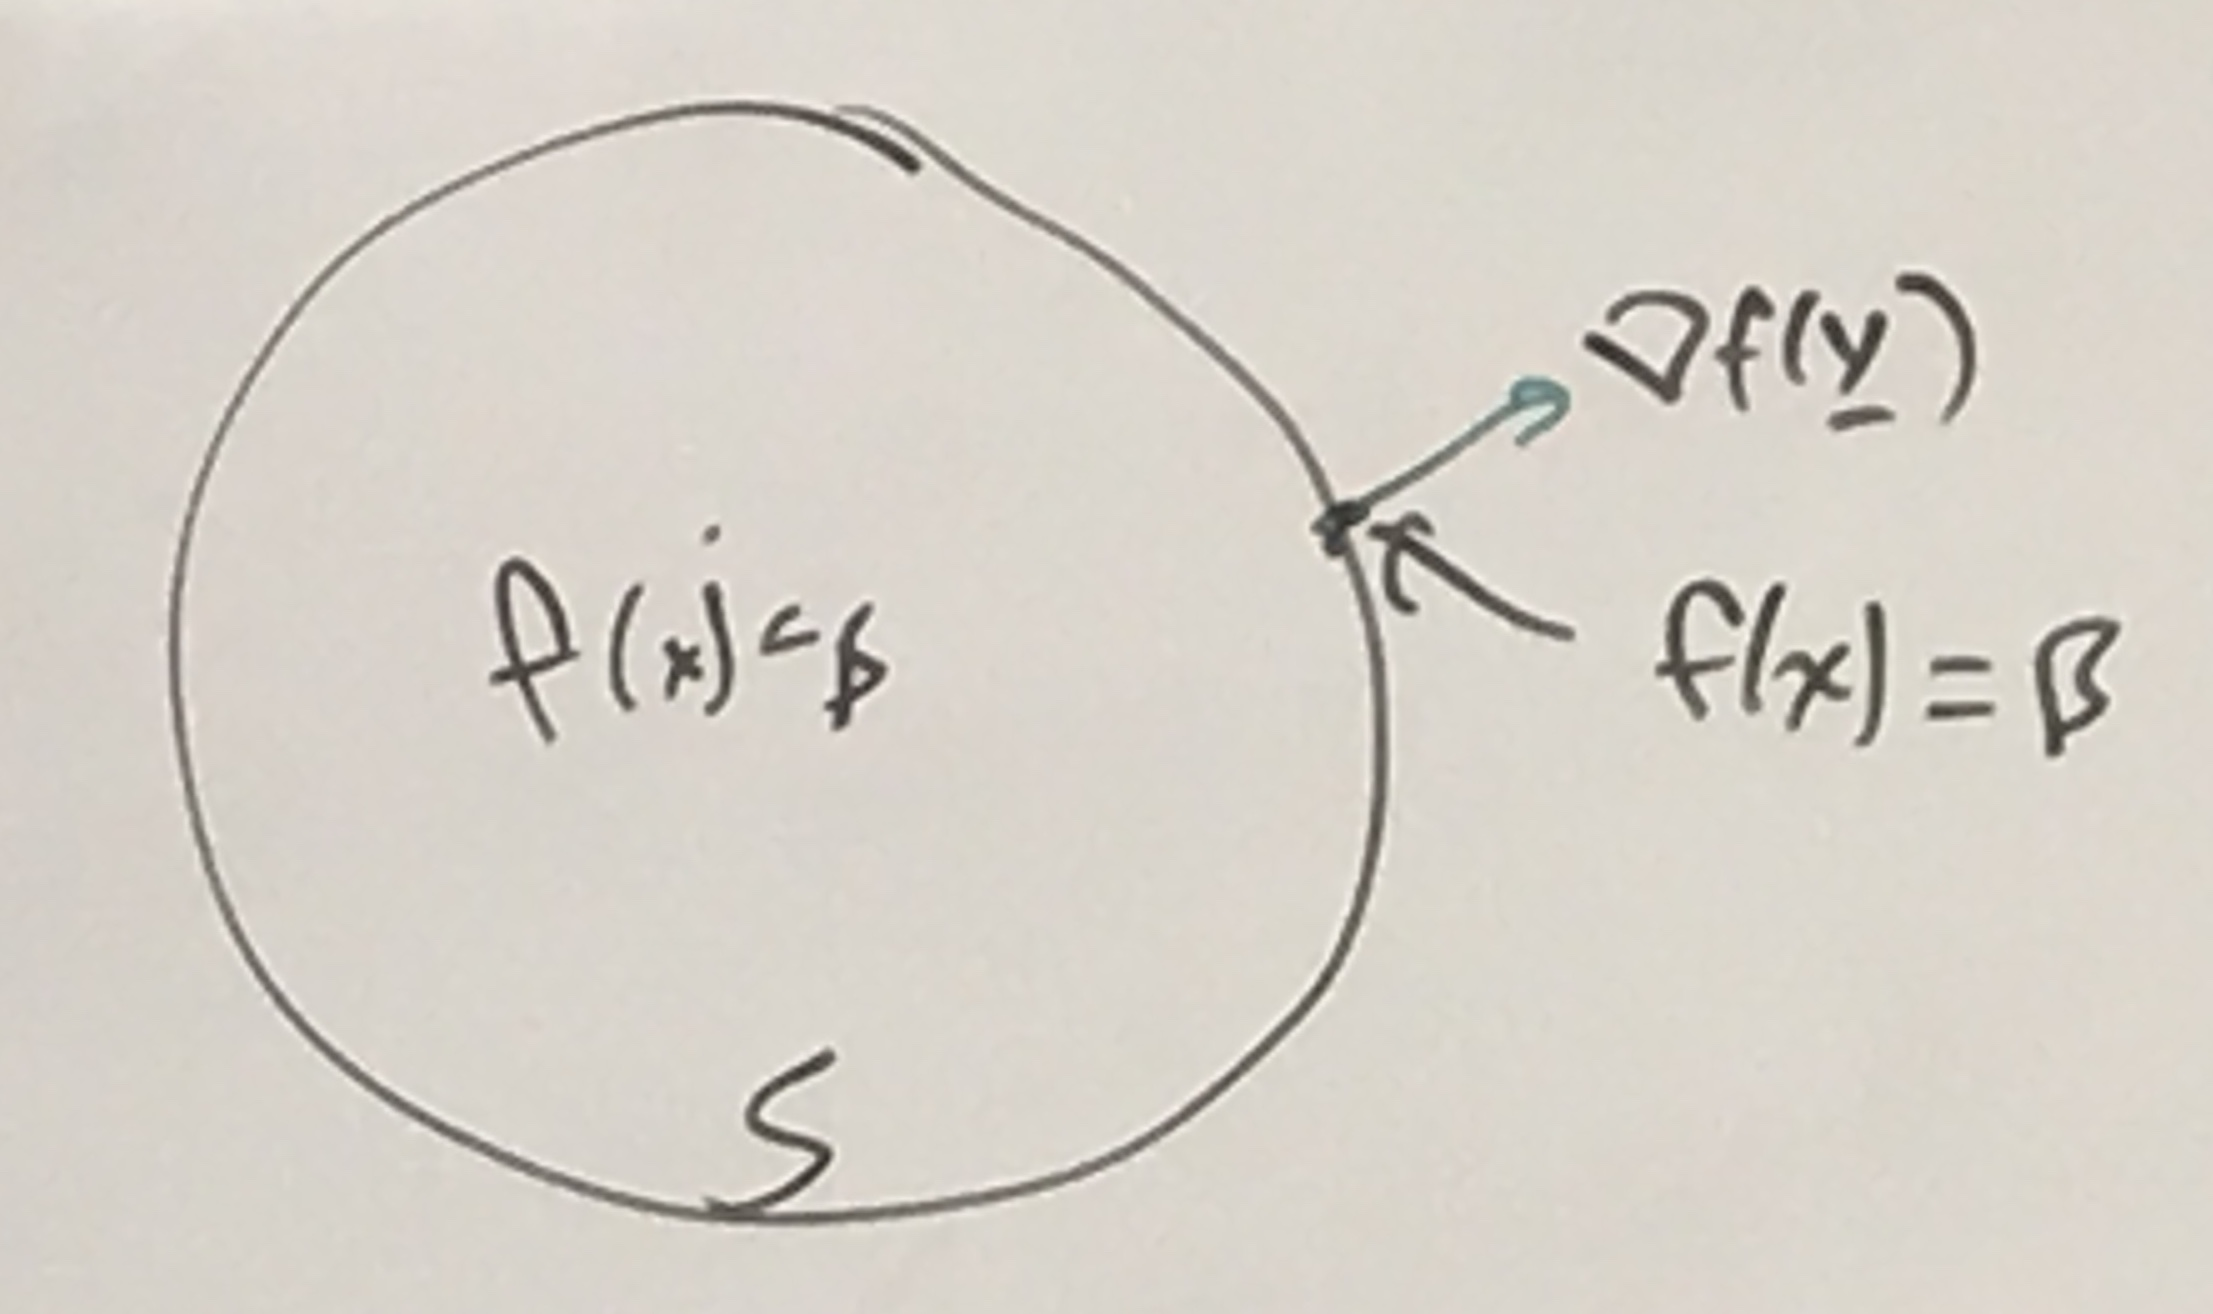
\includegraphics[scale=0.12]{IMG_2387.JPG}
\end{center}

\begin{proof}
    \begin{enumerate}[label=(\alph*)]
        \item Let $f(\vec{x}) < \beta$. Convex functions are continuous on the interior of their domain, thus $\exists r > 0$ such that
        \[
            \forall \vec{y} \in \overline{B}_r(\vec{x}),\, f(\vec{y}) < \beta \implies \overline{B}_r(\vec{x}) \subseteq S
        \]
        So,
        \[
            \vec{v} \in \text{N}_S(\vec{x}) \setminus \left\{\vec{0}\right\} \implies \forall \vec{y} \in S,\, \vec{v}^\top(\vec{y} - \vec{x}) \leq 0.
        \]
        Thus, we take $\vec{y} = \underbrace{\vec{x} + \frac{r\vec{v}}{\|\vec{v}\|}}_{\in \overline{B}_r(\vec{x}) \subseteq S} \leftarrow$ (norm $= r$)

        So,
        \[
            \vec{v}^\top\left(\left(\vec{x} + \frac{r\vec{v}}{\|\vec{v}\|}\right) - \vec{x}\right) \leq 0 \implies r\|\vec{v}\| \leq 0
        \]
        which is impossible. Thus, $\nexists \vec{v} \in \text{N}_S(\vec{x}) \setminus \left\{\vec{0}\right\}$.

        \item $\{\lambda\nabla f(\vec{x}) : \lambda \geq 0\} \subseteq \text{N}_S(\vec{x})$:

        Let $\vec{y} \in S$. Then,
        \begin{align*}
            0 &\underbrace{\geq}_{\text{by def. of } S} f(\vec{y}) - \beta = f(\vec{y}) - f(\vec{x}) \\
            &\geq \nabla f(\vec{x})^\top(\vec{y} - \vec{x}) \tag{subgradient inequality}
        \end{align*}
        So, $\nabla f(\vec{x}) \in \text{N}_S(\vec{x}) \implies \forall \lambda \geq 0,\, \lambda \nabla f(\vec{x}) \in \text{N}_S(\vec{x})$. Thus, $\left\{\lambda\nabla f(\vec{x}) : \lambda \geq 0\right\} \subseteq \text{N}_S(\vec{x})$.

        $\text{N}_S(\vec{x}) = \left\{\lambda\nabla f(\vec{x}) : \lambda \geq 0\right\}$:

        Select $\vec{v} \in \R^n \setminus \{\lambda\nabla f(\vec{x}) : \lambda \geq 0\}$. We aim to show that $\vec{v} \notin \text{N}_S(\vec{x})$.

        We try to find a $\vec{y} \in S$ such that $\vec{v}^\top(\vec{y} - \vec{x}) > 0$, which would imply that $\vec{v} \notin \text{N}_S(\vec{x})$.

        We write $\vec{v} = \lambda\nabla f(\vec{x}) + \vec{d}$, where $\vec{d} \in \nabla f(\vec{x})^\bot$. By our hypothesis, either $\vec{d} \neq \vec{0}$ or $\lambda < 0$.

        In the first case, we construct $\vec{y}$ as $\vec{x} + $ (a certain linear combination of $\vec{d}$ and $\nabla f(\vec{x})$).

        In the second case, we construct $\vec{y}$ as $\vec{x} + $ (some multiple of $\nabla f(\vec{x})$).

        In both cases, we find $\vec{y} \in S$ such that $\vec{v}^\top(\vec{y} - \vec{x}) > 0$, as needed.

        \begin{center}
            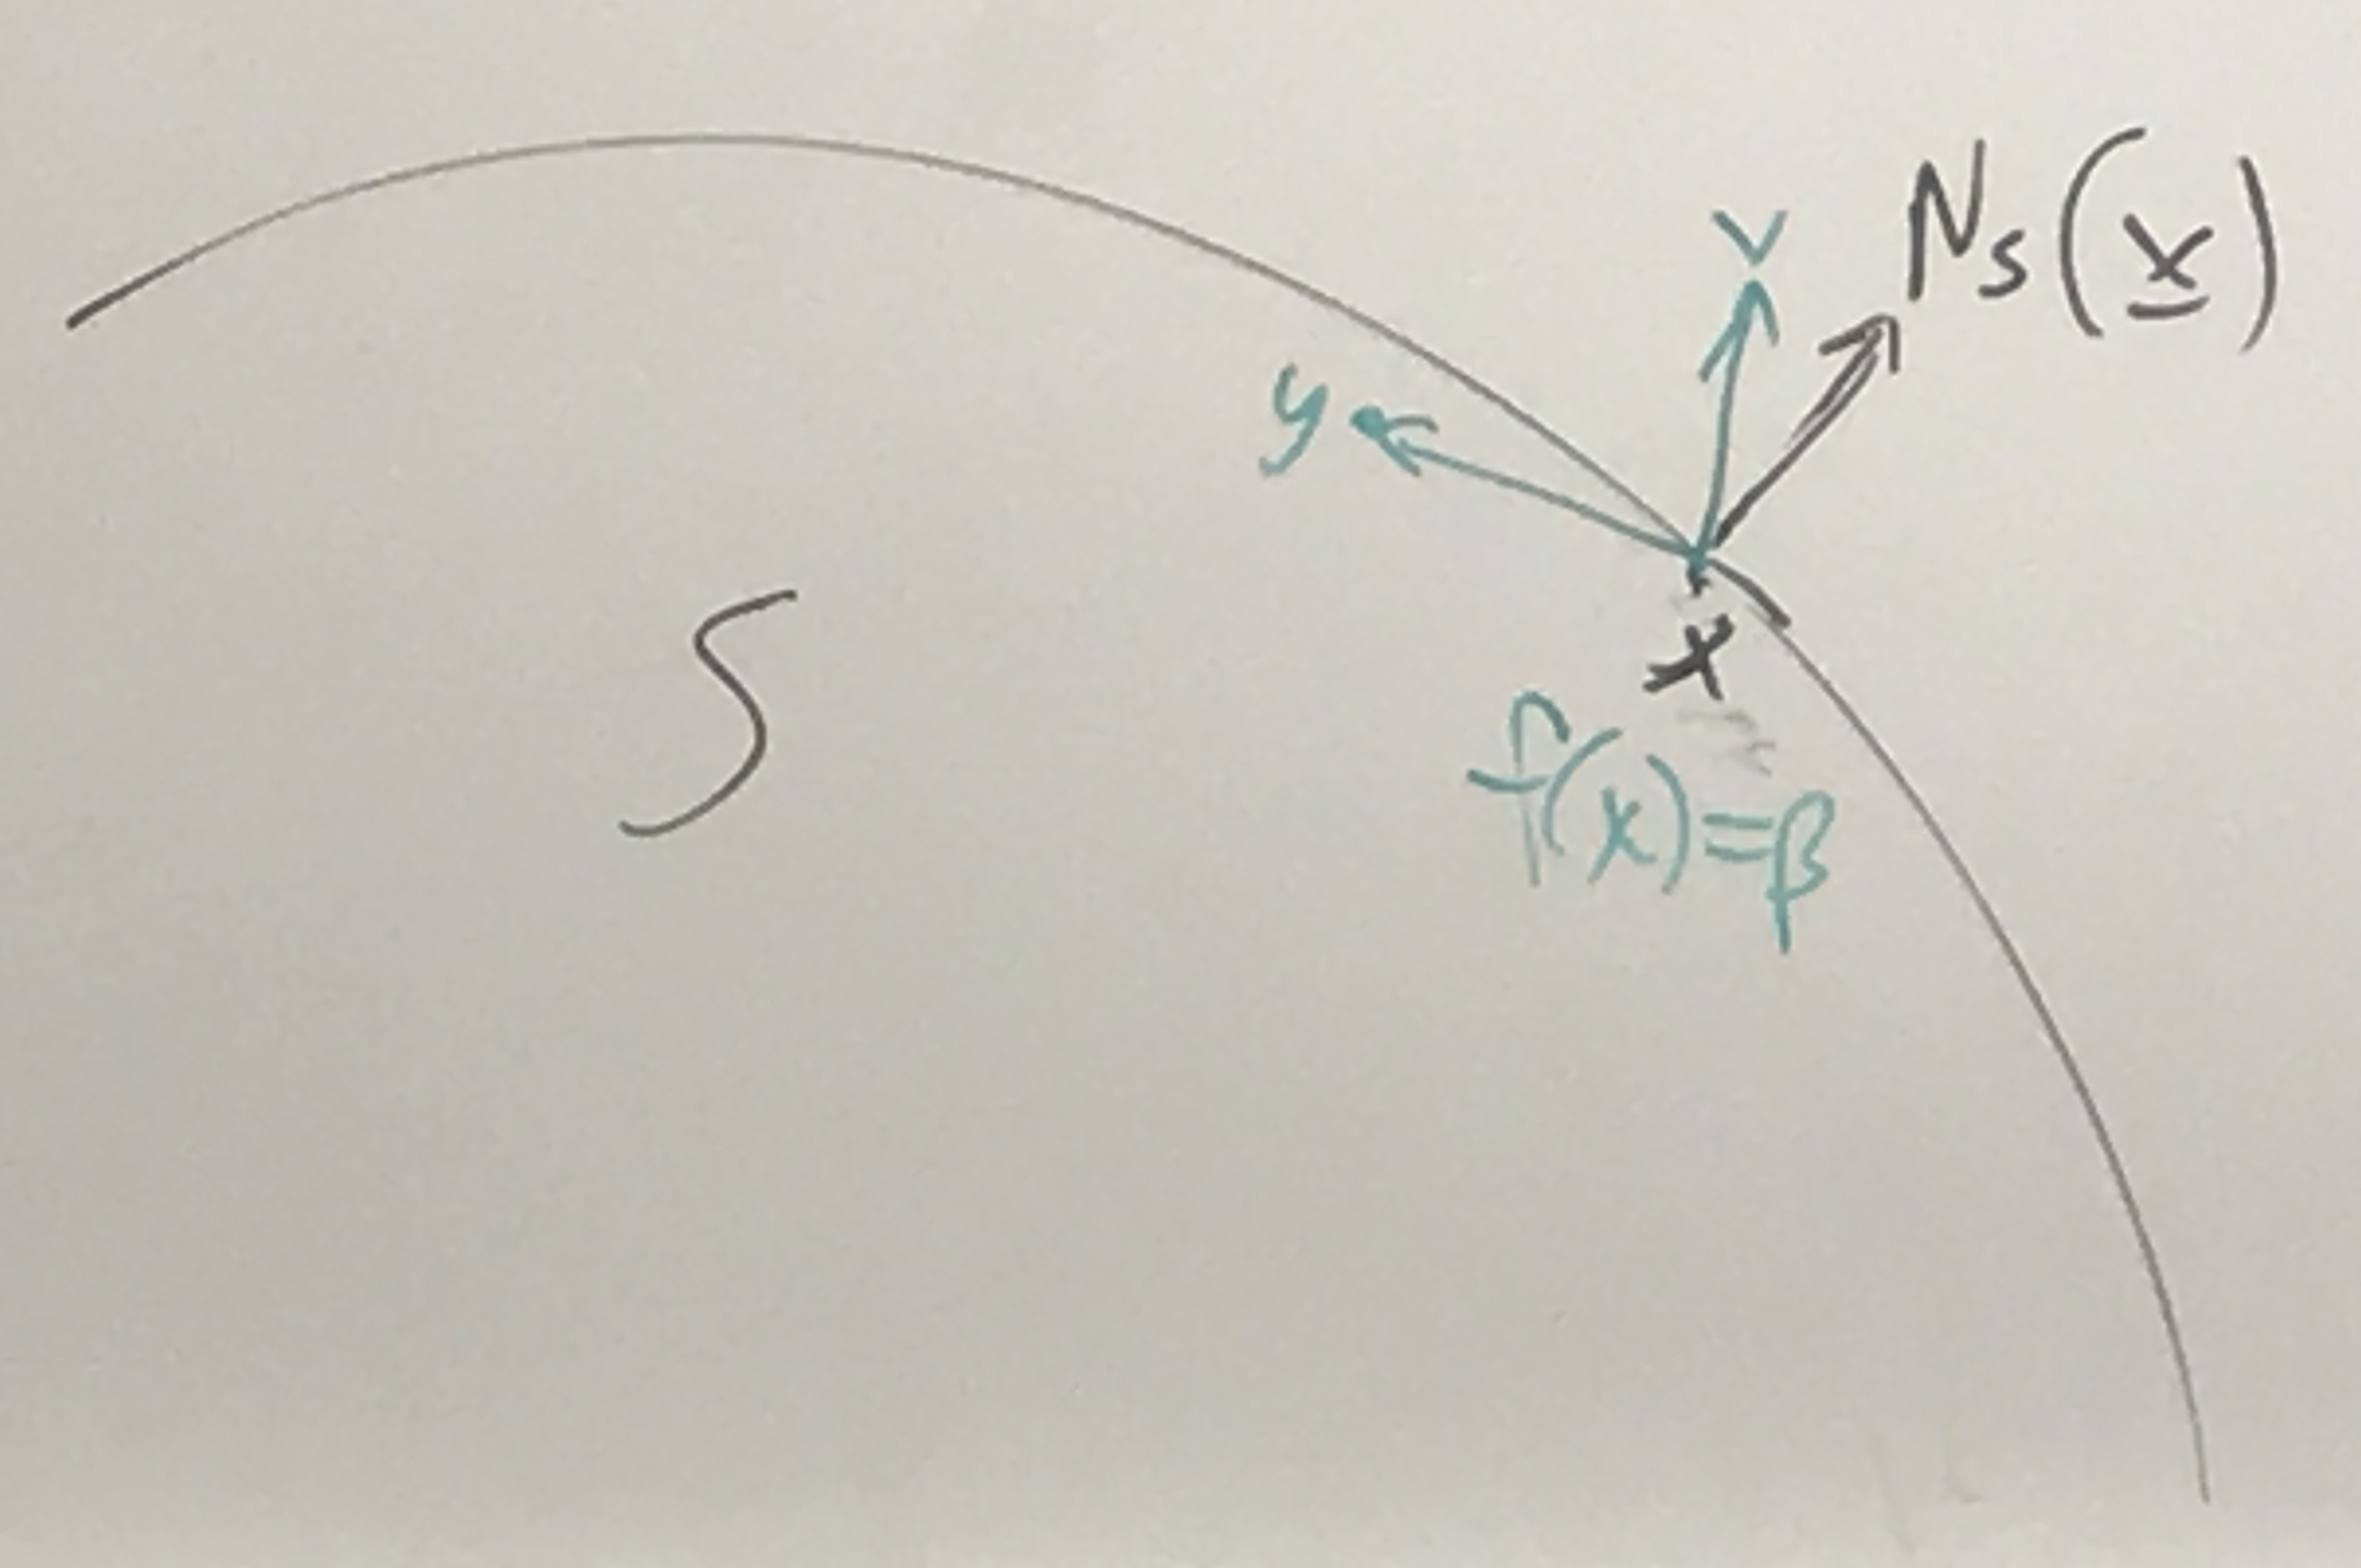
\includegraphics[scale=0.08]{IMG_2388.JPG}
        \end{center}
    \end{enumerate}
\end{proof}

\textbf{Theorem.} (also not in the textbook)

Suppose that $\Omega = \{\vec{x} \in \R^n : A\vec{x} = \vec{b}\} \subseteq \R^n$ where $A \in \mathcal{M}_{m,\, n}(\R)$, and $\vec{b} \in \R^m$ (we call this an affine set). Then, $\forall \vec{x} \in \Omega$, $\text{N}_{\Omega}(\vec{x}) = \text{Range}\left(A^\top\right)$.

\begin{proof}
    \begin{align*}
        \vec{v} \in \text{N}_{\Omega}(\vec{x}) &\iff \underbrace{\forall \vec{y} \in \Omega}_{\text{i.e., } \forall \vec{y} \text{ satisfying } A\vec{y} = \vec{b}},\, \vec{v}^\top(\vec{y} - \vec{x}) \leq 0 \\
        &\iff \forall \vec{w} \in \text{Null}(A),\, \vec{v}^\top\vec{w} \leq 0
        &\hspace{12pt} \rightarrow A\vec{y} = b \iff A\vec{y} = A\vec{x} \iff A(\vec{y} - \vec{x}) = \vec{0}. \\
        &\iff \forall \vec{w} \in \text{Null}(A),\, \vec{v}^\top\vec{w} = 0 \tag{$\vec{w} \in \text{Null}(A) \iff -\vec{w} \in \text{Null}(A)$} \\
        &\iff \vec{v} \in \text{Null}(A)^\bot \\
        &\iff \vec{v} \in \text{Range}\left(A^\top\right) \tag{by the fundamental theorem of linear algebra}
    \end{align*}
\end{proof}

\section{Convex Programming (C.P.)}

\[
    \min\left(f_0(\vec{x})\right)
\]
such that
\[
    f_1(\vec{x}) \leq 0,\, \ldots,\, f_m(\vec{x}) \leq 0,\, \text{and } A\vec{x} = \vec{b}
\]
where $f_0,\, \ldots,\, f_m \colon \R^n \to \R \cup \{\infty\}$ are all convex.

Smooth case: $f_0,\, \ldots,\, f_m$ are all differentiable on an open set containing $\Omega = \{\vec{x} : f_1(\vec{x}) \leq 0,\, \ldots,\, f_m(\vec{x}) \leq 0\}$, the feasible region.

Examples of smooth convex programming:
\begin{itemize}
    \item ($\ell_1$ LS-2)
    \item SVM-4
    \item SVM-6
    \item SVM-7
\end{itemize}

SVM-1:
\[
    \max_{\vec{x},\, \vec{\xi},\, \vec{t}}\left(\{\min(\{t_1,\, \ldots,\, t_N\})\}\right)\, \text{ such that ...}
\]
is equivalent to
\[
    \underbrace{\min_{\vec{x},\, \vec{\xi},\, \vec{t}}}_{\text{min as in (C.P.)}}\left(\{\underbrace{\max(\{-t_1,\, \ldots,\, -t_N\})}_{\text{Convex function of } t_l \text{'s}}\}\right)\, \text{ such that ...}
\]
which is not a smooth and convex function. So, SVM-1 is C.P., not sooth.

\section{KKT Conditions for Smooth C.P.}
For a given $\hat{\vec{x}}$
\begin{enumerate}
    \item $\hat{\vec{x}} \in \Omega$ (primal feasibility)
    \item $\exists \vec{\lambda} \in \R^m$, $\exists \vec{\nu} \in \R^p$ such that
    \begin{enumerate}
        \item $\vec{\lambda} \geq \vec{0}$ (dual feasibility)
        \item $\forall k = 1:m,\, A_kf_k\left(\hat{\vec{x}}\right) = 0$ (complementarity)
        \item $\nabla f_0\left(\hat{\vec{x}}\right) + \sum_{k = 1}^{k = m} \lambda_k \nabla f_k\left(\hat{\vec{x}}\right) + A^\top\nu = \vec{0}$ (gradient equation)
    \end{enumerate}
\end{enumerate}

If $\hat{\vec{x}}$ satisfies 1 and 2, it is called a KKT point.

\textbf{Theorem}. \textit{If $\hat{\vec{x}}$ is a KKT point, then it is a global minimizer of (C.P.)}

\textbf{Theorem}. \textit{Assume a CQ holds. If $\hat{\vec{x}}$ is a global minimizer of (C.P.), then $\hat{\vec{x}}$ is a KKT point.}

Example CQ's
\begin{enumerate}
    \item Polyhedrality: each $f_k$ has the form $f_k(\vec{x}) = \vec{a}_k^\top\vec{x} + b$ where $\vec{a_k} \in \R^n$ and $b \in \R$, OR,
    \item Slater: $\exists \vec{x}_0$ such that $A\vec{x}_0 = \vec{b}$, and $\forall k = 1:m$, $f_k(\vec{x}_k) < 0$.
\end{enumerate}
How to prove this:

$\vec{x}^*$ is optimal for (C.P.) $\iff -\nabla f(\vec{x}^*) \in \text{N}_{\Omega}(\vec{x}^*)$

$-\nabla f(\vec{x}^*) \in \left(\sum_{k = 1}^{k = m} \text{N}_{S_k}(\vec{x}^*)\right) + \text{N}_A(\vec{x}^*)$, where $S_k = \{\vec{x} : f_k(\vec{x}) \leq 0\}$. This requires CQ.

Let $a = \{k \in \{1,\, \ldots,\, m\} : f_k(\vec{x}^*) = 0\}$ (active constraint). Let $\mathcal{I} = \{1,\, \ldots,\, m\} \setminus a$ (inactive constraints $\rightarrow f_k(\vec{x}^*) < 0$).

\begin{align*}
    &\iff -\nabla f(\vec{x}^*) \in \left(\sum_{k \in a} \underbrace{\text{N}_{S_k}(\vec{x}^*)}_{= \{\lambda\nabla f_k(\vec{x}^*) : \lambda \geq 0\}}\right) + \underbrace{\text{N}_A(\vec{x}^*)}_{\text{Range}\left(A^\top\right)} \\
    &\iff -\nabla f(\vec{x}^*) = \sum_{k \in a} \lambda_k \nabla f_k(\vec{x}^*) + A^\top\vec{\nu}, \quad \text{for some } \lambda_k \geq 0 \text{ where } k \in a \text{, and for some } \vec{\nu} \in \R^p. \\
    &\iff -\nabla f(\vec{x}^*) = \sum_{k = 1}^{k = m} \lambda_k \nabla f_k(\vec{x}^*) + A^\top\vec{\nu}, \quad \text{for some } \vec{\lambda} \in \R^m,\, \vec{\lambda} \geq \vec{0} \text{ such that } \forall k \in \mathcal{I},\, \lambda_k = 0, \\
    &\hspace{196pt} \text{and for some } \vec{\nu} \in \R^p.
\end{align*}

In case of equality constraints, theory known to Lagrange (1800s).

In equality constraints (Kuhn \& Tucker 1952), Karush's master's thesis 1930.

\section{Non-smooth Optimization Chapter 8}
Recall the subgradient inequality:

If $f \colon \R^n \to \R \cup \{\infty\}$ is differentiable at $\vec{x} \in \dom(f)$ then
\[
    \forall \vec{y} \in \R^n,\, f(\vec{y}) \geq f(\vec{x}) + \nabla f(\vec{x})^\top(\vec{y} - \vec{x})
\]

\begin{center}
    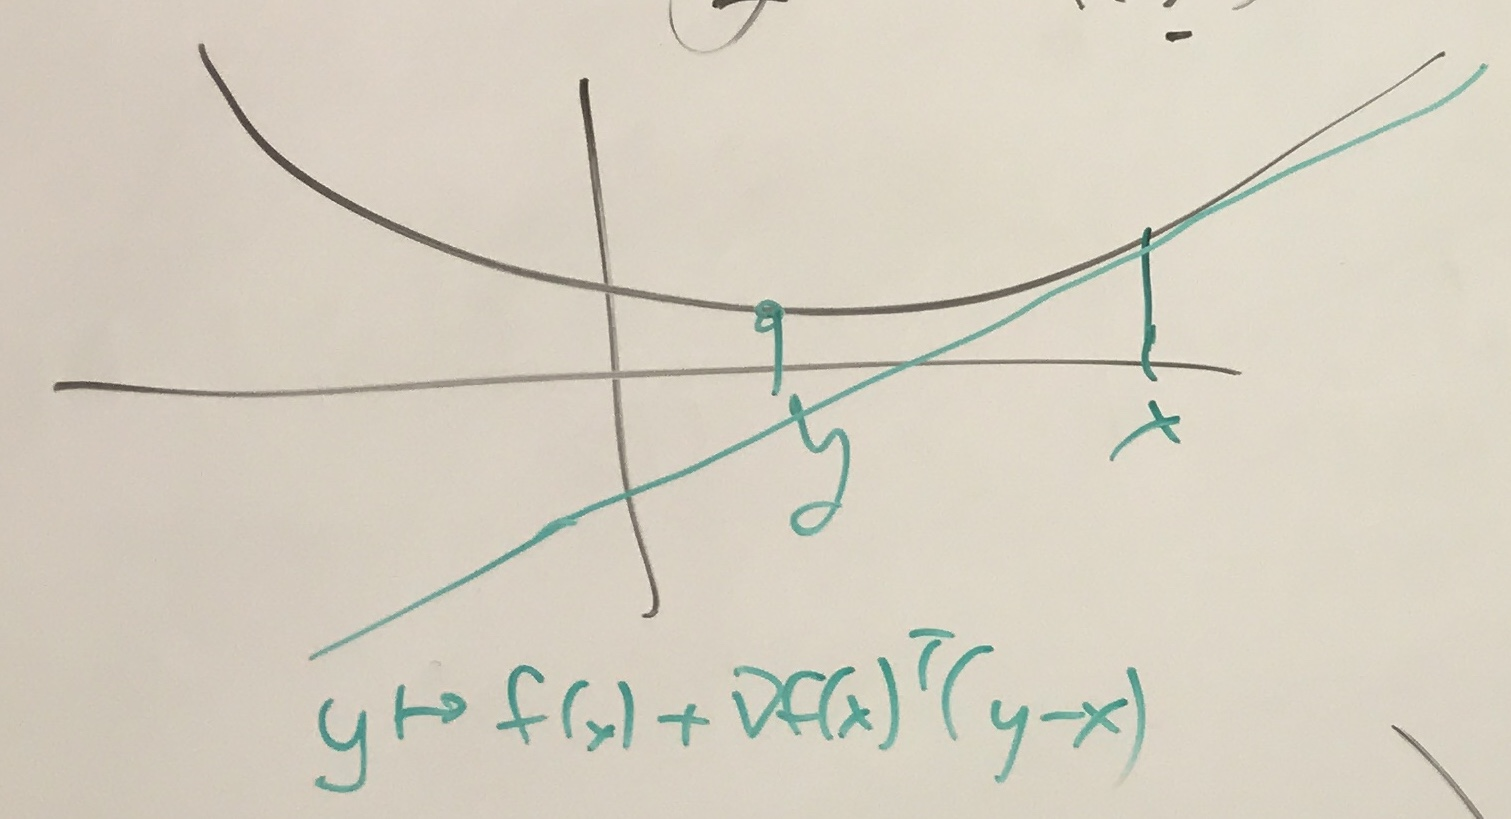
\includegraphics[scale=0.22]{subgrad_ineq.JPG}
\end{center}

What if $f$ is not differentiable, e.g., $f(x) = |x|$:

\begin{center}
    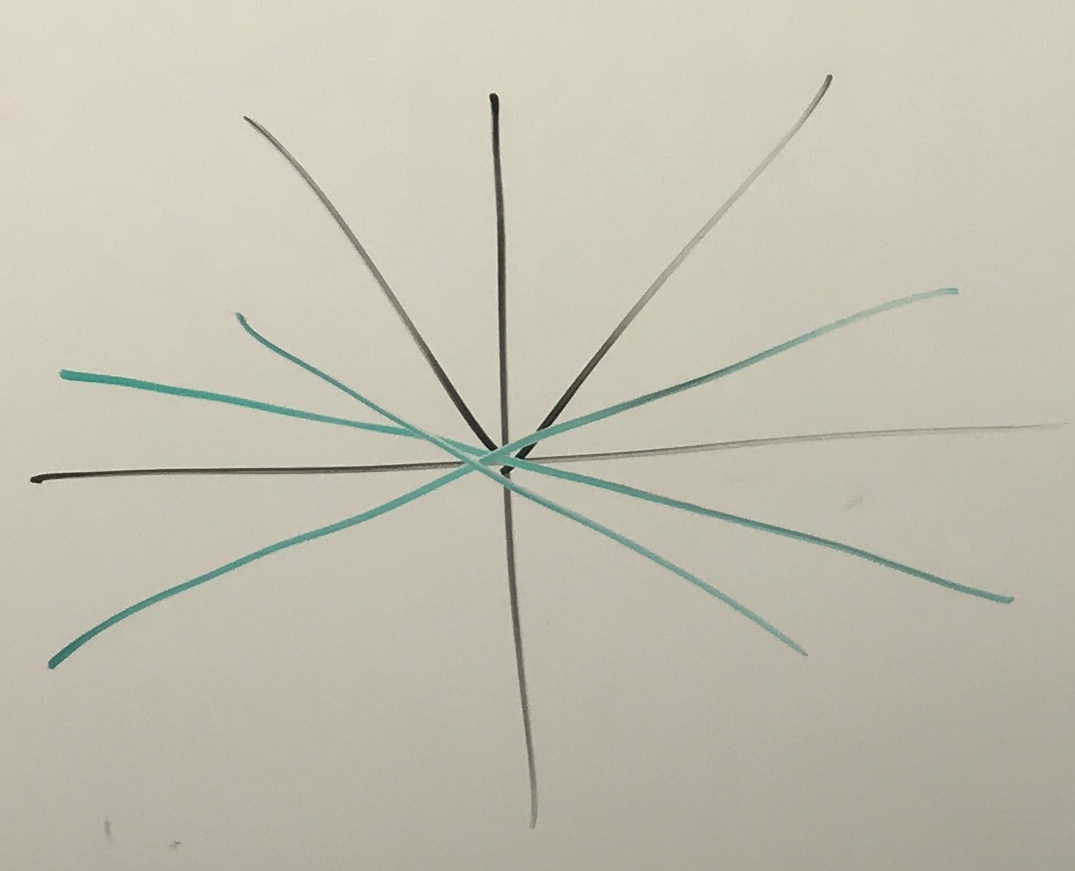
\includegraphics[scale=0.22]{absolute_x.JPG}
\end{center}

We say that $\vec{g} \in \R^n$ is a subgradient of $f \colon \R^n \to \R \cup \{\infty\}$ at $\vec{x} \in \dom(f)$ if $\forall \vec{y} \in \R^n$, $f(\vec{y}) \geq f(\vec{x}) + \vec{g}^\top(\vec{y} - \vec{x})$.

\end{document}
